\chapter{Desarrollo software}

Una vez nos hemos situado en el contexto en el que se ubica este proyecto, y hemos expuesto los objetivos a cumplir y las herramientas necesarias, nos adentramos a explicar en este capítulo las soluciones desarrolladas para llegar a buen puerto.\\

\section{Diseño}

El escenario que se presenta consta de cuatro elementos principales: el drone, el ordenador a bordo, el ordenador remoto y el usuario humano final. El diseño consta de dos conexiones de tal manera que permitan al usuario final poder teleoperar el cuadricóptero: la primera conexión es entre un navegador web en el ordenador local, el cuál irá a bordo del drone, y el propio drone; la segunda conexión es entre este navegador local y un navegador remoto, dónde se creará una interfaz web amigable y de fácil uso para el control a distancia del drone por parte del usuario final.\\

\begin{figure}[h!]
\centering
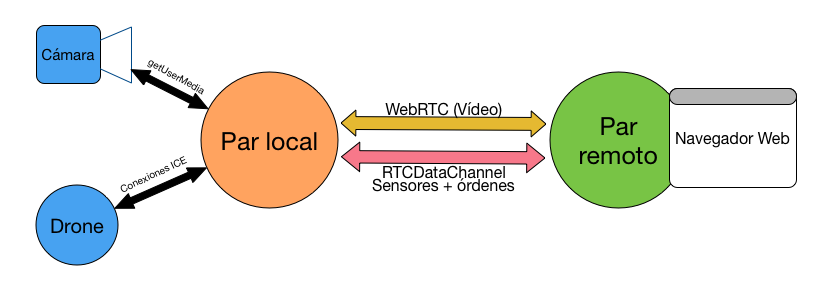
\includegraphics[width=0.9\textwidth]{esquema_general}
\caption{Esquema general del proyecto.}
\label{fig:esquemageneral}
\end{figure}

En la figura \ref{fig:esquemageneral} se representa el esquema general del proyecto con los cuatro actores y las sub-divisiones realizadas. A continuación se expone una vista general a la solución desarrollada para cada uno de esos sub-problemas:

\begin{enumerate}[(a)]

\item \textbf{Conexión local: }consta de dos conexiones: se ha utilizado la API \emph{getUserMedia} de WebRTC para acceder a las imágenes de una cámara que también irá a bordo del drone; por otro lado se ha establecido la conexión entre el drone y el navegador utilizando el plugin ICEJS, el cuál nos permite conectarnos con interfaces ICE a través de \emph{websockets} en el navegador.

\item \textbf{Conexión entre navegadores:} Una conexión punto a punto entre navegadores con la API \emph{RTCPeerConnection} para transferir las imágenes de la cámara, y la API \emph{RTCDataChannel} para transferir los datos de los sensores y las órdenes dadas. 

\item \textbf{Cliente web}: trabaja como transductor para representar los datos recibidos de los sensores del drone y la cámara por un lado, y por el otro de recoger y enviar las órdenes de vuelo dadas por el usuario final.
\end{enumerate}


De manera general en cuanto a la estructura global el par local deberá establecer la conexión con el drone, acceder a sus sensores y actuadores y a la cámara. Deberá también establecer una conexión con el ordenador remoto y enviarle todos estos datos obtenidos del drone. Del par remoto recibirá las órdenes y comandos de movimiento, que deberá enviárselos al drone.\\

El par remoto deberá establecer la conexión con el par local. De éste recibirá todos los datos del drone y deberá representarlos de una manera que el usuario final pueda conocer la situación de vuelo del drone en cada momento. Deberá tener una interfaz amigable que le permita recoger las órdenes de movimiento dadas por el usuario, y enviárselas al par local.\\

Como primer problema se presentó decidir cuál de los dos ordenadores que necesitamos para la conexión WebRTC sería el que realizaría la llamada y en qué momento del flujo. Éste no es un problema trivial, ya que la selección de uno u otro haría que el desarrollo de la aplicación fuese completamente distinto.\\

Se optó por que el par que lleva la batuta de la conexión fuese el ordenador local, ya que éste a su vez también es el encargado de  establecer la conexión con el drone. De esta manera tenemos un par que es el que actuará de maestro, estableciendo ambas conexiones en los momentos oportunos.\\

Como ya se comentó en la sección \ref{sec:senalizacion} el momento en el que se envía y se recibe cada paquete de información es crítico en este sistema de señalización de oferta/respuesta, por lo que el flujo de la comunicación se diseñó y se ha desarrollado como se muestra en la figura \ref{fig:flujodellamada}.\\


\begin{figure}[h!]
\centering
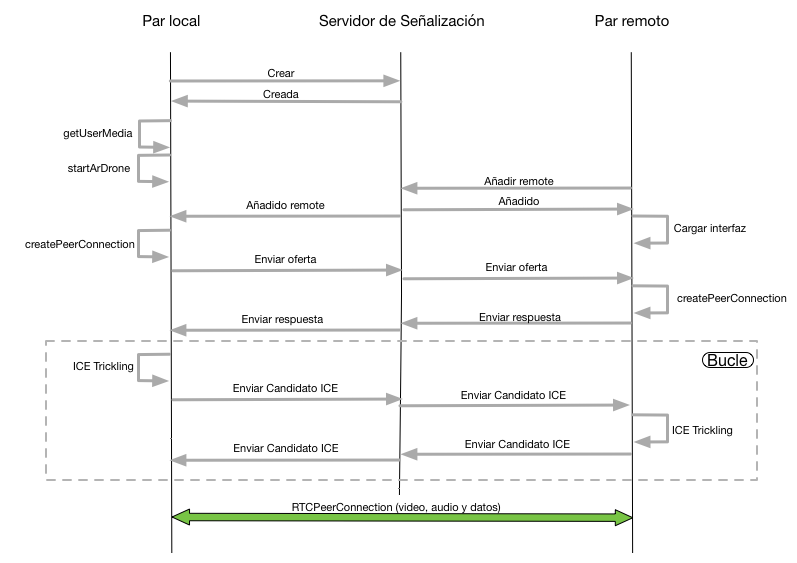
\includegraphics[width=1.1\textwidth]{diagrama_general}
\caption{Flujo de llamada del proyecto}
\label{fig:flujodellamada}
\end{figure}

Como se puede observar el par local es el que lleva la iniciativa de la conexión. En primer término inicia la comunicación con el servidor de señalización. Una vez que éste le contesta afirmativamente a su mensaje de creación de la comunicación inicia un proceso en el que se conecta al cuadricóptero y accede a la cámara. Una vez realizados estos dos procesos espera a que un par remoto quiera unirse a la conexión.\\

Cuando el par remoto accede al servidor de señalización, éste le envía un mensaje al par local indicando que un par remoto se ha conectado. En este momento el par local inicia la creación de la conexión \emph{RTCPeerConection} de WebRTC. Primero se produce el intercambio de paquetes SDP a través del servidor de señalización, y posteriormente el de ICE. Una vez finalizados ambos ya tenemos establecida la conexión WebRTC entre ambos pares.\\

\section{Conexión local drone-navegador}

Esta parte la hemos solucionado dividiendo el problema en dos sub-problemas. Por un lado la conexión con el servidor encargado de conectarse al cuadricóptero, \emph{ardrone\_server}. A través de esta conexión seremos capaces de conectarnos a los elementos, sensores y actuadores del drone. Por otro obtener un flujo de vídeo para poder visualizarlo en la parte remota. Este problema lo hemos solucionado incorporando una cámara a bordo del drone que irá conectada al par local y a la cual accederemos desde el navegador con la API \emph{getUserMedia} que nos brinda WebRTC.\\

Se explica a continuación la conexión con el servidor y posteriormente el acceso a la cámara con \emph{getUserMedia}.\\


\subsection{ArDrone\_server y WebSockets}\label{subsec:ardrone}

Para establecer la conexión con el drone se ha utilizado el componente \texttt{ardrone\_server} de JdeRobot. Este componente son dos piezas. Un plugin en Gazebo para el drone simulado, y el servidor \texttt{ardrone\_server} para el drone real. Estas dos piezas cuentan con las mismas interfaces de conexion ICE por lo que con un único desarrollo es posible utilizar indistintamente tanto la versión simulada con Gazebo como el drone real.\\

Esta conexión se ha divido en dos partes, servidor y cliente. En la parte de servidor se ha tratado su configuración y la activación de \emph{WebSockets} como protocolo sobre el que van mensajes ICE, y la parte del cliente se ha desarrollado desde cero el código \emph{JavaScript} necesario para establecer y controlar la conexión.\\

\subsubsection{Servidor}

Los componentes JdeRobot utilizan, como ya hemos visto, interfaces ICE para el intercambio de información del que se ocupan. Los navegadores no tienen capacidad de usar el \emph{middleware} ICE directamente. Para poder conectarnos con estas interfaces ICE hemos tenido que instalar el plugin ICE for JavaScript, o ICE\-JS. Este plugin nos habilita la opción de conectarnos a estas interfaces directamente desde el navegador usando \emph{websockets}.\\

Aunque estaba disponible la versión 3.6 de ICE\footnote{https://doc.zeroc.com/display/Ice36/Home} la cuál trae en la \emph{suite} instalado de serie ICE\_JS, hemos usado la versión 3.5, ya que es la versión compatible con la versión actual de JdeRobot\footnote{http://jderobot.org/Manual-5}. En esta versión ICE\_JS es un plugin el cuál hay que instalarlo descargando el código fuente desde la página de Zeroc\footnote{https://zeroc.com} y compilarlo.\\

Una vez instalado hay que activar este plugin en el servidor ICE. Para ello hay que añadir la siguiente línea en el archivo de configuración del servidor ICE, en nuestro caso \emph{ardrone\_server}:\\

\begin{lstlisting}[caption=Activación del plugin ICEJS]
# ICE-JS
Ice.Plugin.IceWS=IceWS:createIceWS
\end{lstlisting}

Posteriormentes, en el mismo archivo hay que indicarle las direcciones IP y los puertos de cada interfaz de conexión. Cada conexión se corresponderá con un \emph{WebSocket}, y la nomenclatura es la siguiente:\\

\begin{lstlisting}[caption=Formato \emph{endpoints} de los \emph{WebSocket} de ICEJS]
# ICE-JS
:ws -h ip -p puerto
\end{lstlisting}


El servidor tiene hasta un máximo de seis interfaces diferentes a las que te puedes conectar. Cada una de estas interfaces nos ofrece un servicio diferente. Para nuestro proyecto hemos usado cuatro de esas interfaces:\\

\begin{itemize}
\item \textbf{Pose3D:} Con esta interfaz accedemos a los datos de orientación y posición del cuadricóptero (x, y, z, h y \emph{quaternion}).
\item \textbf{Navdata:} Esta interfaz nos proporciona los datos de navegación procedentes de los sensores, como la velocidad de las componentes (x, y, z) del drone, altitud, la velocidad del viento, el nivel de batería, etc.
\item \textbf{CMDVel:} Esta interfaz es la encargada de recibir las órdenes de movimiento.
\item \textbf{BaseExtra:} Esta interfaz nos da funcionalidades extra como las órdenes de aterrizaje o de despegue del cuadricóptero.
\end{itemize}

Así pues, esta es la forma final que tiene nuestro archivo de configuración:\\

\begin{lstlisting}[caption=Archivo de configuración de ArDrone\_Server.]
# Ice-JS
Ice.Plugin.IceWS=IceWS:createIceWS

# Variables de control para ver traceroutes de las conexiones ICE.
#Ice.Trace.Network = 3
#Ice.Trace.Protocol=1


ArDrone.Pose3D.Endpoints=default -h 0.0.0.0 -p 9998:ws -h 0.0.0.0 -p 19000
ArDrone.Pose3D.Name=ardrone_pose3d

ArDrone.RemoteConfig.Endpoints=default -h 0.0.0.0 -p 9997
ArDrone.RemoteConfig.Name=ardrone_remoteConfig

ArDrone.Navdata.Endpoints=default -h 0.0.0.0 -p 9996:ws -h 0.0.0.0 -p 15000
ArDrone.Navdata.Name=ardrone_navdata

ArDrone.CMDVel.Endpoints=default -h 0.0.0.0 -p 9995:ws -h 0.0.0.0 -p 11000
ArDrone.CMDVel.Name=ardrone_cmdvel

ArDrone.Extra.Endpoints=default -h 0.0.0.0 -p 9994:ws -h 0.0.0.0 -p 17000
ArDrone.Extra.Name=ardrone_extra

ArDrone.NavdataGPS.Endpoints=default -h 0.0.0.0 -p 9993
ArDrone.NavdataGPS.Name=ardrone_navdatagps
\end{lstlisting}

A parte de los \emph{endpoints} es también importante configurar correctamente el nombre de cada uno de las interfaces, ya que será necesario para una correcta conexión desde el navegador. La dirección ip \texttt{0.0.0.0} indica que la dirección de escucha del servidor es la ip local del equipo. Se puede también observar que hemos creado únicamente \emph{WebSockets} para las cuatro interfaces anteriormente descritos.\\


\subsubsection{Cliente}

Una vez configurado el servidor hemos creado el método \texttt{ArDrone.js} en el navegador local, el cuál es el encargado de conectarse y manejar la conexión con el servidor \texttt{ardrone\_server}.\\

Para establecer una comunicación ICE lo primero que se ha creado han sido las variables ICE necesarias. Estas han sido creadas de la siguiente manera:\\

\begin{lstlisting}[caption=Variables para la conexión ICE.]
// Variable ICE para la conexion
var id = new Ice.InitializationData();
id.properties = Ice.createProperties();
id.properties.setProperty("Ice.Trace.Network", "3"); // Propiedad para tracear la conexion
id.properties.setProperty("Ice.Trace.Protocol", "1"); // Propiedad para tracear la conexion
var communicator = Ice.initialize(id);
\end{lstlisting}

Por si fallase la comunicación ICE se le ha añadido a la variable \emph{id} una propiedad con la que podemos seguir la ruta de la comunicación y detectar en qué punto se produce el fallo.\\

Posteriormente es necesario crear una variable que actuará como \emph{proxy}. Es necesario crear una variable por cada interfaz a la que necesitemos conectarnos. Esta es la nomenclatura que sigue:\\

\begin{lstlisting}[caption=Nomenclatura de variable que actuará como \emph{proxy}]
var proxy = communicator.stringToProxy("nombre_interfaz:ws -h " + ip + " -p " + "puerto");
\end{lstlisting}

Nótese en la nomenclatura que donde pone \emph{nombre\_interfaz} se corresponde con el nombre que le hemos asignado al \emph{endpoint} en el archivo de configuración del servidor. Asimismo el puerto también se corresponde con el configurado.\\


La comunicación con las interfaces se realiza mediante el objeto promesa o \emph{promise} de JavaScript. Este objeto se usa para las comunicaciones asíncronas y se caracteriza por tener tres estados: pendiente, cumplida o rechazada. Cuando una promesa ha sido llamada puede presentar el estado cumplida o rechazada, lo que nos permite llamar al argumento correspondiente y poder actuar en consonancia. De esta manera podemos hacer que métodos asíncronos actúen como métodos síncronos.\\

El núcleo de la conexión con el servidor \emph{ardrone\_server} queda como sigue:\\
\newpage
\begin{lstlisting}[caption=Núcleo ArDrone]
// base extra connection
var baseextra = communicator.stringToProxy("ardrone_extra:ws -h " + ip + " -p " + baseextraPort);
jderobot.ArDroneExtraPrx.checkedCast(baseextra).then(
    function(ar){
        extraProxy = ar;
        console.log("extraProxy connected: " + ar);
    },
    function(ex, ar){
        console.log("extraProxy NOT connected: " + ex);
    }
);               

// NavData
var basenavdata = communicator.stringToProxy("ardrone_navdata:ws -h " + ip + " -p " + navdataProxyPort);
jderobot.NavdataPrx.checkedCast(basenavdata).then(
    function(ar){
        console.log("navdataProxy connected: " + ar);
        navdataProxy = ar;
        navdataProxy.getNavdata().then(
        function(navdata){
            if (navdata.vehicle == ARDRONE_SIMULATED) {
                virtualDrone = true;
                console.log("virtualDrone = true");
            } else {
                virtualDrone = false;
                console.log("virtualDrone = false");
            }
        },
        function (ex, ar){
            console.log("Fail getNavdata() function: " + ex);
        }
        );
    },
    function (ex, ar){
        console.log("navdataProxy NOT connected: " + ex);
    }        
);        

// CMDVelPrx
var basecmdVel = communicator.stringToProxy("ardrone_cmdvel:ws -h " + ip + " -p " + cmdVelProxyPort);
jderobot.CMDVelPrx.checkedCast(basecmdVel).then(
    function(ar){
        console.log("cmdVelProxy connected: " + ar);
        cmdVelProxy = ar;
    },
    function(ex, ar){
        console.log("cmdVelProxy NOT connected: " + ex);
    }
);             

// Pose3D
var basepose3D = communicator.stringToProxy("ardrone_pose3d:ws -h " + ip + " -p " + pose3DProxyPort);
jderobot.Pose3DPrx.checkedCast(basepose3D).then(
   function(ar){
       console.log("pose3DProxy connected: " + ar);
       pose3DProxy = ar;
        window.po = pose3DProxy;
        resolve("Stuff worked!");
       pose3DProxy.getPose3DData().then(
           function (ar){
               console.log("getPoseDData().");
               pose = ar;
           },
           function(ex, ar){
               console.log("Fail call getPoseDData().");
           });
   },
   function(ex, ar){
       console.log("pose3DProxy NOT connected: " + ex)
   }
);
\end{lstlisting}

Tenemos cuatro promesas con sus respectivos argumentos de éxito o fallo, una para cada interfaz ICE. Las variables que nos devuelven los argumentos de éxito se guardan en las variables correspondientes de cada interfaz \texttt{(extraProxy, navdataProxy, cmdVelProxy, pose3DProxy)}. Estas variables son importantes ya que son las que utilizaremos en las funciones manejadoras que se explican a continuación.\\

En este punto ya estamos conectados con las interfaces del servidor, y por consiguiente, con el drone. Para poder teleoperar el drone hay que crear unas funciones que serán los manejadores. Por un lado hemos creado las funciones en JavaScript de aterrizaje y de despegue. Estas funciones utilizan la interfaz \emph{ardrone\_extra}:\\

\begin{lstlisting}[caption=Funciones aterrizaje y despegue.]
// extraProxy functions  
function takeoff() {
    extraProxy.takeoff().then(
        function(ar){
            console.log("Take Off.");
        },
        function(ex, ar){
            console.log("Take Off failed.")
        }
     );
}
    
function land() {
        extraProxy.land().then(
        function(ar){
            console.log("Landing.");
        },
        function(ex, ar){
            console.log("Landing failed: " + ex)
        }
     );
}
\end{lstlisting}

Ejecutar estas órdenes en el drone se realiza en JavaScript también con el objeto promesa, con sus respectivos argumentos de éxito o error en la ejecución de la misma.\\

Las interfaces ICE \emph{Navdata} y \emph{Pose3D} son las encargadas de suministrar todos los datos de navegación de los sensores. Las funciones JavaScript con las que accedemos a estas interfaces y actualizamos todos estos datos son las siguientes:

\begin{lstlisting}[caption=Variables actualización datos de los sensores.]
function updateNavData() {
    navdataProxy.getNavdata().then(
        function(ar){
            navdata = ar;
            //console.log("updateNavData()");
        },
        function (ex, ar){
            console.log("Fail getNavdata() function." + ex)
        }        
    );    
}

function updatePose(){
    pose3DProxy.getPose3DData().then(
            function (ar){
                pose=ar;
                //console.log("getPose3DData. ")
            },
            function(ex, ar){
                console.log("Fail call getPoseDData(): " + ar);
            });   
}
\end{lstlisting}


Llamando a estas funciones periódicamente tenemos actualizados en todo momento los datos de navegación procedentes de los sensores: brújula, posición, velocidad, altitud...\\

Para poder teleoperar el drone se ha implementado una función que es la encargada de enviarle las órdenes de movimiento. Estas órdenes nos llegan desde el par remoto a través de la conexión entre nevagadores que explicaremos con mas detenimiento más adelante.\\

\begin{lstlisting}[caption=Función manejadora de las órdenes.]
function sendVelocities () {
    cmdVelProxy.setCMDVelData(cmd).then(
        function(ar){
          //console.log("sendVelocities.");
        },
        function(ex, ar){
          console.log("sendVelocities failed.")
        }
    );
}
\end{lstlisting}

Esta función admite una variable como argumento, (\emph{cmd}) la cuál contiene los parámetros que recibimos del drone. Esta variable es una variable CMDVel de JdeRobot y tiene esta estructura:\\

\begin{lstlisting}[caption=Variable CMD]
var cmd = new jderobot.CMDVelData; 
cmd.linearX=0.0;
cmd.linearY=0.0;
cmd.linearZ=0.0;
cmd.angularZ=0.0;
cmd.angularX=0.0;
cmd.angularY=0.0;
\end{lstlisting}

Contiene seis parámetros que son las velocidades lineales X, Y, Z y las angulares en los mismos ejes. Estas velocidades pueden variar desde 0.0 hasta 1.0 en intervalos de 0.1.\\


\subsection{getUserMedia}

La interfaz que no hemos utilizado de las que nos ofrece el servidor \texttt{ardrone\_server} es la interfaz \emph{cameraserver}. Esta interfaz se encarga de recoger las imágenes de la cámara integrada en el drone. La razón por la que no usar la interfaz del drone que accede a la cámara es que queríamos utilizar la tecnología que nos brinda WebRTC con drones, y esto incluye el acceso a una cámara con la API \emph{getUserMedia}. Esta cámara se conecta a nuestro ordenador local a través de una conexión USB. Cámara y MiniPC van a a bordo del drone.\\

Como WebRTC aún no es una norma, para acceder a la cámara desde cualquier navegador debemos crear una variable que sea compatible con todos los que tengan implementado las APIs de WebRTC. Para ello hay que añadirle los prefijos correspondientes de cada navegador:\\


\begin{lstlisting}[caption=Variable de getUserMedia.]
navigator.getUserMedia = navigator.getUserMedia || navigator.webkitGetUserMedia || navigator.mozGetUserMedia;
\end{lstlisting}


Acceder a la cámara  con \emph{getUserMedia} se hace a través de una función que admite tres argumentos. El primer argumento que admite la función es una variable en la que le indicamos las restricciones que queremos: audio, vídeo, solo uno de ellos, resoluciones... Las configuraciones para nuestro proyecto son las siguientes:\\

\begin{lstlisting}[caption=Restricciones de getUserMedia]

var constraints = {
    audio: false,
    video: {
        width: { ideal: 1280, max: 1920 },
        height: {ideal: 720, max: 1080 },
    }
};

\end{lstlisting}

Sólo accedemos al vídeo de la cámara, ya que el audio no lo necesitamos para el proyecto. Por otro lado indicamos una resolución ideal, de 1280x720 píxeles. Si la cámara que le conectamos al ordenador tiene más capacidad restringimos su resolución a HD (1920x1080 píxeles).\\

Los siguientes dos argumentos son dos llamadas de vuelta o \emph{callbacks}. El primero es el callback de éxito, y el segundo el de error. Según sea de exitoso el acceso a la cámara se llamará a una función u otra. Si nos devuelve éxito se llama a una función con la que guardaremos el flujo y lo visualizaremos en un elemento vídeo de HTML5. Esta visualización que se produce en el par local no es necesaria pero se ha incluido para tenerlo como referencia a la hora de realizar los experimentos. Si devuelve error mostramos en el terminal del navegador un mensaje del error ocurrido.\\

\begin{lstlisting}[caption={getUserMedia.}, label={lst:getusermedia}]
// Manejador de exito
function handleUserMedia(stream){
	localStream = stream;

	if (window.URL){
		localVideo.src = window.URL.createObjectURL(stream);
	} else{
		localVideo.src = stream;
	}
	//console.log('Adding local stream.');
	// Envio un mensaje al servidor como ack de exito al llamar gerUserMedia()	
}

// manejador de error
function handleUserMediaError(error){
	console.log('getUserMedia error: ', error);
}

//Funcion getUserMedia
navigator.getUserMedia(constraints, handleUserMedia, handleUserMediaError); 
\end{lstlisting}

El flujo que nos proporciona \emph{getUserMedia} y el cuál guardamos en la variable \emph{localStream} (línea 3 del listado \ref{lst:getusermedia}) será el que enviemos al par remoto con la API \emph{RTCPeerConnection}. Este punto lo veremos en la sección \ref{subsec:transmisionvideo}.\\

\section{Conexión entre navegadores}

Interconectar el ordenador remoto al drone a través del ordenador local es el segundo de los objetivos marcados. Para ello vamos a utilizar WebRTC por su comunicación entre pares sin necesidad de utilizar servidores intermedios.\\

Este objetivo se ha divido en tres sub-objetivos como siguen:
\begin{itemize}

\item \emph{Visualización en remoto de cámara a bordo:} La conexión tiene que ser capaz de transportar el flujo audiovisual de la cámara del drone desde el navegador local hasta el navegador remoto.

\item \emph{Sensores de navegación.} Los datos obtenidos de los sensores de navegación del cuadricóptero como la brújula, el GPS, altímetro... deberán ser enviados al ordenador remoto donde se visualizarán.

\item \emph{Órdenes}. Desde el ordenador remoto deberán enviarse hacia el ordenador local las órdenes dadas para el aterrizaje, despegue, y comandos de movimiento.

\end{itemize}

Para desarrollar la conexión multimedia entre los navegadores con la tecnología WebRTC lo primero que se ha desarrollado ha sido el servidor de señalización.\\

\subsection{Servidor de señalización}

Las necesidades a cubrir en cuanto al servidor de señalización es que sea capaz de intercambiar los datos de red necesarios (Candidatos ICE) y de paquetes SDP. El intercambio debe hacerse con el protocolo de oferta/respuesta según lo establecido en la arquitectura JSEP explicada con anterioridad.\\

Se ha optado por desarrollar el servidor escrito sobre \emph{Node.js}\footnote{https://nodejs.org/}. Las razones por las que hemos elegido este servidor es que está escrito en JavaScript, por lo que nos resulta muy útil al utilizarse el mismo lenguaje de programación que vamos a utilizar para el resto del proyecto. Por otro lado es un servidor muy liviano.\\

Para cumplir con la arquitectura JSEP vamos a utilizar la librería \emph{Socket.io}\footnote{http://socket.io}, la cuál nos facilita el desarrollo de aplicaciones con necesidades de conexión entre equipos a través de \emph{Websockets}.\\

Como se puede ver en la figura \ref{fig:flujodellamada}, el servidor recibe cuatro tipos de paquetes diferentes. Cuando se conecta el par local, cuando se conecta el par remoto, intercambio de candidatos ICE e intercambio de SDP. Sabiendo que tanto los candidatos ICE como los paquetes SDP son objetos, decidimos crear el servidor aceptando tres tipos diferentes de paquetes: el inicial del par local, el inicial del par remoto, y mensajes genéricos que contendrían los objetos anteriormente mencionados. Así pues, esta es la forma del código que gestiona en el servidor el intercambio de paquetes para la señalización.\\

\begin{lstlisting}[caption=Núcleo servidor de señalización]
io.sockets.on('connection', function (socket){

	// Manejador de mensajes genericos 'message' (intercambios SDP y Candidatos ICE)
	socket.on('message', function (message) {
		//log('Server --> got message: ', message);
		// Si el que envia es Droner hay que mandarlo al remote
		if (socket.id == dronerID) {
			io.sockets.socket(newPeer).emit('message', message);
		// Si el que envia es remote hay que mandarselo al droner
		} else if (socket.id== newPeer) {
			io.sockets.socket(dronerID).emit('message', message);
		} 
	});

	// manejador de mensjes 'create'  enviados por Droner
	socket.on('create', function () {
		//log('Server --> Droner has sido conectado');
		socket.join();
		dronerID = socket.id;
		socket.emit('created');
	});
	

	// Manejador de mensajes 'join remote ' enviados por remote
	socket.on('join remote', function () {
		//log("Server --> Un 'remote' se ha unido.");
		
		io.sockets.in().emit('join remote');
		socket.join();
		newPeer = socket.id;
		socket.emit('joined');
	});
});
\end{lstlisting}

Una vez tenemos el servidor operativo vamos a explicar cómo se ha creado la conexión entre pares y cómo se ha usado esta conexión para transmitir el vídeo de la cámara y los datos de los sensores del drone hasta el par remoto.\\

\subsection{RTCPeerConnection: Transmisión de vídeo}\label{subsec:transmisionvideo}

La conexión entre pares se crea en el momento en el que el par local recibe del servidor de señalización un mensaje indicando que el par remoto se ha conectado y está preparado para establecer la conexión. En ese momento se ejecuta una función que configura los parámetros necesarios y  crea la comunicación.\\

Al igual que en \emph{getUserMedia} debemos configurar las variables necesarias para que sean compatibles con todos los navegadores. Para establecer la conexión necesitamos tres variables distintas:\\


\begin{lstlisting}[caption=Variables WebRTC]
RTCPeerConnection = window.RTCPeerConnection || window.mozRTCPeerConnection || 
                       window.webkitRTCPeerConnection || window.msRTCPeerConnection;
RTCPSessionDescription = window.RTCSessionDescription || window.mozRTCSessionDescription ||
                       window.webkitRTCSessionDescription || window.msRTCSessionDescription;
RTCIceCandidate = window.RTCIceCandidate || window.mozRTCIceCandidate ||
                        window.webkitRTCIceCandidate || window.msRTCIceCandidate;
\end{lstlisting}


\begin{itemize}
\item \emph{RTCPeerConnection}: Esta variable es la encargada de crear y mantener la conexión entre pares. Esta variable necesitará de las otras dos para crear la conexión.
\item \emph{RTCPSessionDescription}: Crea los SDP locales y se encarga de gestionar los SDP recibidos.
\item \emph{RTCIceCandidate}: Encargada de descubrir los Candidatos ICE y de gestionar los recibidos del otro par.
\end{itemize}


También debemos indicarle los servidores STUN y TURN a los que conectarse para averiguar los pares de IP y puerto para los Candidatos ICE:\\

\begin{lstlisting}[caption=Servidores STUN y TURN]
var ICE_config = {
  'iceServers': [
    {
      'urls': 'stun:stun.l.google.com:19302'
    },
    {
      'urls': 'stun:23.21.150.121'
    },
    {
      'urls': 'turn:192.158.29.39:3478?transport=udp',
      'credential': 'JZEOEt2V3Qb0y27GRntt2u2PAYA=',
      'username': '28224511:1379330808'
    },
    {
      'urls': 'turn:192.158.29.39:3478?transport=tcp',
      'credential': 'JZEOEt2V3Qb0y27GRntt2u2PAYA=',
      'username': '28224511:1379330808'
    }
  ]
};
\end{lstlisting}

Una vez tenemos las variables configuradas, la forma en la que creamos la conexión WebRTC es la siguiente:\\

\begin{lstlisting}[caption=RTCPeerConnection.]

var PeerConnection = new RTCPeerConnection(ICE_config, pc_constraints);
\end{lstlisting}

Esta función admite dos argumentos. El primero es la configuración ICE que acabamos de ver y el segundo es una variable con las restricciones de todas las funcionalidades y configuraciones que tiene \emph{RTCPeerConnection}. En nuestro caso esa variable está vacía ya que la configuración por defecto es más que adecuada para nuestros intereses.\\

Para el intercambio de paquetes en la señalización es necesario crear los manejadores que \emph{RTCPeerConnection} necesita para los SDP y para los Candidatos ICE. El par local tiene sus manejadores ya que es el encargado de llevar la batuta de la conexión, y el par remoto tiene otros manejadores diferentes. \\

Los SDP se manejan en el par local con el método \emph{createOffer} que al ser llamado activa el proceso de crear la oferta SDP. Cada vez que crea uno nuevo salta un evento en la función que se le ha indicado, llamada \emph{gotLocalDescription}. Esta función se encarga de ajustar el SDP local al SDP que se acaba de crear y de mandárselo al otro par a través del servidor de señalización. Si al crear un SDP se produce un error se llama a la función de error, la cual se encargará de notificarlo en la consola del navegador.\\


\begin{lstlisting}[caption={Manejador de los SDP.}, label={lst:manejadorsdp}]
// Funcion de exito
function gotLocalDescription(sessionDescription){
  PeerConnection.setLocalDescription(sessionDescription, successLocalSDP, errorLocalSDP);
  sendMessage(sessionDescription);
}

// Funcion de error
function onSignalingError(error){
  console.log('Fallo al crear el SDP: ' + error);	
}

// Metodo manejador de las SDP
PeerConnection.createOffer(gotLocalDescription, onSignalingError);
\end{lstlisting}

Esta oferta es recibida en el par remoto a través del servidor de señalización y se guarda como la oferta del otro par, ya que la necesitaremos para conocer las características del flujo audiovisual que nos llegará:\\


\begin{lstlisting}[caption={Estableciendo SDP del par remoto.}]
PeerConnection.setRemoteDescription(new RTCPSessionDescription(message));
\end{lstlisting}

Al establecer el SDP remoto ocurre un evento del método \emph{createAnswer} y crea una respuesta a la oferta recibida.\\

\begin{lstlisting}[caption=Manejador de respuestas SDP]
PeerConnection.createAnswer(gotLocalDescription, onSignalingError);
\end{lstlisting}


Las funciones de éxito y error \emph{gotLocalDescription} y \emph{onSignalingError} son las mismas que en el otro par, puedes encontrarlas en el listado \ref{lst:manejadorsdp}.\\

Para manejar los Candidatos ICE utilizamos el método manejador \emph{onicecandidate}, el cuál llama a la función indicada, \emph{handleIceCandidate()} en nuestro caso, en el momento en que se encuentra un Candidato ICE. Esta función se encarga de enviar el candidato a través del servidor de señalización. Ambos pares usan este mismo evento con la misma configuración en la detección y envío de candidatos ICE.\\

\begin{lstlisting}[caption=Manejador de los Candidatos ICE locales.]
function handleIceCandidate(event){
  //console.log('handleIceCandidate event: ', event);
  if (event.candidate) {
    sendMessage({
    type: 'candidate',
    label: event.candidate.sdpMLineIndex,
    id: event.candidate.sdpMid,
    candidate: event.candidate.candidate});
  } else {
    console.log('End of candidates.');
  }
    // console.log('Local ICE candidate: \n' + event.candidate.candidate);
  
}

// Metodo manejador de candidatos ICE
PeerConnection.onicecandidate = handleIceCandidate; // Manejador ICE local (manda ICE local a remoto)
\end{lstlisting}

Los candidatos son recibidos en ambos pares a través del servidor de señalización. Se crea el candidato y se le añade como candidato remoto con el método \emph{addIceCandidate}.\\

\begin{lstlisting}[caption=Manejador de los Candidatos ICE remotos.]
var candidate = new RTCIceCandidate({sdpMLineIndex:message.label,candidate:message.candidate});
PeerConnection.addIceCandidate(candidate);
\end{lstlisting}


Uno de los puntos mas importantes para el proyecto que se tiene que encargar \emph{RTCPeerConnection} es transferir el flujo visual desde el par local al par remoto. WebRTC nos lo permite de una forma muy sencilla. En el par local, con un método al que le añadimos como argumento el flujo que hemos obtenido al llamar a la API \emph{getUserMedia}:\\

\begin{lstlisting}[caption=Manejador del flujo audiovisual en el par local.]
PeerConnection.addStream(localStream); 
\end{lstlisting}

Y en el par remoto con un método manejador llamado \emph{onaddstream}, que en el momento en el que salta el evento llama a la función \emph{handleRemoteStreamAdded}, y ésta se encarga de configurar el flujo en una etiqueta vídeo de HTML5.\\

\begin{lstlisting}[caption=Manejador del flujo audiovisual en el par remoto.]
// Funcion manejadora
function handleRemoteStreamAdded(event) {

    var remoteVideo = document.getElementById("droneVideo"); // 

	if (window.URL){
		remoteVideo.src = window.URL.createObjectURL(event.stream);
	} else{
		remoteVideo.src = event.stream;
	}
    //console.log('Remote stream attached!!.');
	remoteStream = event.stream;
}

// Metodo manejador 
PeerConnection.onaddstream = handleRemoteStreamAdded;
\end{lstlisting}

Una vez creada y establecida la conexión \emph{RTCPeerConnection} la usaremos para crear la conexión de datos \emph{RTCDataChannel}, para transportar toda la información necesaria en ambas direcciones.\\


\subsection{RTCDataChannel}

\emph{RTCDataChannel} nos permite transferir cualquier tipo de dato u objeto entre los pares a través de la comunicación creada por \emph{RTCPeerConnection}. Hemos usado esta API para transferir tanto los datos obtenidos de los sensores del drone (del navegador local al navegador remoto) como las órdenes de movimiento dadas (deo navegador remoto al navegador local).\\

Para crear esta conexión basta con llamar al método \emph{createDataChannel()} de \emph{RTCPeerConnection} en el par local ya que es quien arranca la conexión. Este método admite dos argumentos, el primero es el nombre que le damos a esta conexión y el segundo es un objeto en el que se especifica la configuración de las propiedades disponibles. La única propiedad que se ha configurado distinta de las que vienen por defecto es la entrega ordenada de paquetes, estableciéndolo en falso, ya que de esta manera introduce menos retraso a la comunicación, eliminando cuellos de botella ya que el medio en el que se transfieren los paquetes no es ruidoso ni tiene condiciones extremas para que se produzcan demasiadas pérdidas de paquetes.\\

\begin{lstlisting}[caption=Establecimiento conexión RTCDataChannel en el par local.]
// Creacion de la comunicacion dataChannel
dataChannel = PeerConnection.createDataChannel("droneDataChannel", {ordered: false});

// Metodo de error para la creacion del dataChannel
dataChannel.onerror = function (error) {
  console.log("Data Channel Error:", error);
};\end{lstlisting}

Si en el momento de crear la conexión ocurre un error salta un evento en el método \emph{onerror} que nos comunica a través de la terminal el error concreto que se ha producido.\\

Para el control de la comunicación RTCDataChannel utiliza tres métodos para gestionar la conexión. Por un lado los métodos de inicio y final de la conexión creada, y el método que maneja los mensajes recibidos.\\

\begin{lstlisting}[caption={Manejadores de RTCdataChannel.}, label={lst:manejadoresdatachannel}]
function handleReceiveChannelStateChange() {
  var readyState = dataChannel.readyState;
  if (readyState == closed) {
    isChannelRunning = false;
    clearInterval(intervalo); //Paramos el intervalo de actulizacion con el drone si el canal se cierra
  }
}

dataChannel.onopen = handleReceiveChannelStateChange;
dataChannel.onclose = handleReceiveChannelStateChange;
dataChannel.onmessage = handleMessage;
};\end{lstlisting}

La función \emph{handleMessage} es la encargada de manejar los mensajes recibidos, pero hablaremos en profundidad de ella más adelante.\\

En el par remoto para establecer la conexión RTCDataChannel hemos configurado el método \emph{ondatachannel}. Este método se encarga de unirse a la comunicación creada por el par local con las mismas propiedades y configuraciones que se le han indicado. Cuando se activa este método llama a la función \emph{gotReceiveChannel} que es la encargada de manejar  la conexión. Esta función se encarga de configurar la conexión en la variable local, y de establecer en los métodos de apertura y cierre de la comunicación las funciones manejadoras. Las función manejadora \emph{handleSendChannelStateChange} es la misma que la mostrada en el listado \ref{lst:manejadoresdatachannel}.\\

\begin{lstlisting}[caption={Establecimiento de RTCDataChannel en el par remoto.}]
function gotReceiveChannel(event) {
	dataChannel = event.channel; // Establece el datachannel
	dataChannel.onopen = handleSendChannelStateChange;
	dataChannel.onclose = handleSendChannelStateChange;
	dataChannel.onmessage = handleMessage;
}

// Evento manejador al recibir apertura comunicacion datachannel del par local.
PeerConnection.ondatachannel = gotReceiveChannel;
};\end{lstlisting}

Una vez establecida la comunicación de datos \emph{RTCDataChannel} podemos enviar los datos a través del método \emph{dataChannel.send()} y recibirlos con el método manejador \emph{onmessage}. A continuación vamos a ver cómo hemos utilizado estos métodos para enviar y recibir los sensores del drone y las órdenes de movimiento.\\


\subsubsection{Sensores de navegación}

Los datos de los sensores los recogemos en el par local. Llamamos a una función del método ArDrone, explicado en la sección \ref{subsec:ardrone}, que a su vez llama a las funciones que se conectan directamente con las interfaces ICE de \texttt{ardrone\_server} para recoger los datos. Esta llamada la hacemos de manera periódica con una función \emph{setinterval()} de JavaScript.\\

\begin{lstlisting}[caption=Intervalo actualización y envío de datos de los sensores.]
intervalo = setInterval(arDrone.updateAndSend, 15);
\end{lstlisting}

Después de actualizar los datos, esta función a su vez llama a la función \emph{sendNavigationData(pose, navdata)} que es la encargada de enviar estos datos a través de la conexión \emph{RTCDataChannel}. Esta función admite dos argumentos, el primero es el objeto \emph{pose}, que contiene los datos recogidos de la interfaz \emph{Pose3D}, y el segundo el objeto \emph{Navdata}, con los datos de navegación recogidos de la interfaz \emph{Navdata}.\\

\begin{lstlisting}[caption=Envio de los datos de los sensores en el par local.]
function sendNavigationData(pose, navdata) {
	var s = {pose:pose, navdata:navdata};
	dataChannel.send(JSON.stringify(s));
	//console.log("Send navigationData.");
}
};\end{lstlisting}

Para enviar los datos al navegador remoto primero creamos un objeto JavaScript, en el que introducimos los objetos \emph{Pose} y \emph{Navdata}. Este objeto lo transformamos a un objeto JSON\footnote{http://www.json.org} para enviarlo por el canal de datos \emph{RTCDataChannel}.\\

Los datos llegan al par remoto en forma de evento a la función \emph{handleMessage()}.\\

\begin{lstlisting}[caption=Manejo de los datos de los sensores en el par remoto.]
function handleMessage(event) {
    var data = JSON.parse(event.data);
    pose = data.pose;
    navdata = data.navdata;
}
\end{lstlisting}

Esta función se encarga de reconvertir el objeto JSON recibido a objeto JavaScript, y posteriormente guardamos los objetos \emph{pose} y \emph{navdatas} para su posterior representación en pantalla. Estos datos los visualizaremos en unos relojes de navegación, los cuáles estudiaremos con más detalle en la sección \ref{subsec:relojesnavegacion}.\\


\subsubsection{Órdenes de movimiento}\label{subsec:ordenes}

El par remoto es el encargado de transferir las órdenes dadas por el usuario al par local, y éste a su vez al drone. El usuario tiene distintas maneras de introducir o hacer saber al equipo las órdenes que quiere dar. Una de ellas es a través de unos \emph{joysticks} multidispositivo situados en las esquinas inferiores de la pantalla, y la otra mediante un mando conectado por USB al ordenador.\\

En la sección \ref{subsec:joysticks} se analizarán en profundidad ambos, mientras que en esta sección nos centraremos en el intercambio de los datos.\\

La forma en la que hemos diseñado la interfaz hace que tengamos dos joysticks, uno de ellos controla la dirección y velocidad del drone, y el otro controla la altitud y el giro del drone. A parte de esto tenemos otro tipo de órdenes, las llamadas especiales, que son la orden de despegue y la orden de aterrizaje. Por este motivo se han creado tres tipos de funciones de envío:\\

\begin{lstlisting}[caption=Funciones de envío de órdenes en el par remoto.]
function enviarOrden(d){
    //console.log(d);
    var data = {orden:d};
    dataChannel.send(JSON.stringify(data));
}

function sendCMDVel(x, y){
    var data = {x:x,y:y};
    //console.log(data);
    dataChannel.send(JSON.stringify(data));
}

function sendAltYaw(alt, yaw){
    //console.log(d);
    var data = {alt:alt, yaw:yaw};
    dataChannel.send(JSON.stringify(data));
}
\end{lstlisting}

La función \emph{enviarOrden()} es llamada al pulsar un botón de despegue o aterrizaje que implementaremos en la interfaz de usuario. En esta función creamos un objeto JavaScript con la orden, le reconvertimos a un objeto JSON y se envía a través del canal RTCDataChannel con \emph{dataChannel.send(JSON.stringify(data));}.\\


\emph{sendCMDVel()} es llamada cuándo el usuario interactúa con el \emph{joystick} situado en la parte inferior izquierda de la pantalla. Esta función admite como argumento el valor de las componentes espaciales \emph{x} e \emph{y}. Creamos un objeto JavaScript y lo enviamos de la misma forma que el resto de datos que enviamos a través del canal RTCDataChannel.\\

Con el segundo \emph{joystick} situado en la esquina inferior derecha controlamos la altitud y el giro del drone. La función \emph{sendAltYaw()} también admite dos argumentos, la altura (o componente espacial \emph{z}) y el giro del drone. Enviamos de la misma manera, creando una variable JavaScript con ellas, reconvertimos a objeto JSON y enviamos \emph{dataChannel.send()}.\\

Todos estos datos los recibimos en el par local con la función \emph{handleMessage()}. En esta función reconvertimos el objeto JSON a objeto JavaScript y llamamos a la función manejadora \emph{handleReceiveData()} a la que le enviamos como argumento el objeto JavaScript.\\

\begin{lstlisting}[caption=Manejo de las órdenes recibidas en el par local.]
// Manejador de datos recibidos 
function handleReceiveData(data) {
  if ("orden" in data) {
    if (data.orden == "takeoff") {
      arDrone.takeoff();
    } else if (data.orden == "land") {
      arDrone.land();
    } else {
      console.log("Orden no valida. ");
    }
  } else if ("x" in data) {
    arDrone.setXYValues(data.x, data.y);
  } else if ("alt" in data) {
    arDrone.setAltYaw(data.alt, data.yaw);
  } else {
    console.log("Dato invalido. ");
  }		
}

// Recibimos los paquetes del datachannel y los enviamos al manejador de datos
function handleMessage(event) {
  //console.log('Received message: ' + event.data);
  var data = JSON.parse(event.data);
  handleReceiveData(data);
}
\end{lstlisting}


La función manejadora se encarga de discernir qué tipo de dato ha llegado y llamar a la función correspondiente del módulo ArDrone.\\

En este punto tenemos toda la comunicación de datos entre pares terminada, por lo que procedemos a explicar el desarrollo de la interfaz web de usuario.\\

\section{Interfaz web de usuario en cliente remoto}

El diseño de la interfaz se ha diseñado con tecnologías web de ultima generación que nos permiten teleoperar el drone de una forma fácil, sencilla e intuitiva.\\

Esta interfaz está compuesta principalmente por cuatro ingredientes: la visualización del vídeo recibido del navegador remoto a pantalla completa, unos \emph{joysticks} virtuales para el manejo del drone complementados con un mando físico, unos relojes de navegación que nos representarán los datos recibidos de los sensores del drone y una visualización espacial en 3D del drone.\\

\subsection{Visualización del vídeo}

Para teleoperar el drone de una manera efectiva necesitamos poder visualizar el vídeo que recibimos de la cámara de la mejor manera posible. Hemos optado por visualizarlo a pantalla completa en el navegador, por debajo del resto de elementos que tendremos en la pantalla. Este tipo de representación es especialmente útil cuándo se ejecuta en un teléfono móvil o en una tableta.\\

Para situar el vídeo a pantalla completa primero necesitamos definir en la hoja de estilos o \emph{CSS} el cuerpo de la página con margen cero, y posteriormente situar el vídeo en el centro de la pantalla y con tamaño 100\%. Para el tiempo que transcurre entre que se inicia el período de señalización hasta que recibimos el vídeo se establece una imagen de fondo\\

\begin{lstlisting}[caption=Vídeo a pantalla completa.]
body{
       background: url(background.jpg) no-repeat;
       background-size: 100% 100%;
}

video#droneVideo { 
       position: fixed;
       top: 50%;
       left: 50%;
       min-width: 100%;
       min-height: 100%;
       width: auto;
       height: auto;
       z-index: -100;
       -webkit-transform: translateX(-50%) translateY(-50%);
       transform: translateX(-50%) translateY(-50%);
       background: url(background.jpg) no-repeat;
       background-size: cover; 
}
\end{lstlisting}

En la figura \ref{fig:interfazweb} se puede observar el vídeo procedente de la cámara mostrándose de fondo por debajo del resto de elementos de la interfaz.\\

\subsection{Joysticks y Gamepad}\label{subsec:joysticks}

Para que el usuario controle el drone hemos optado por desarrollar dos opciones. La primera opción es a través de unos \emph{joysticks} situados en la pantalla, los cuáles son multidispositivo, ya que se pueden usar en un ordenador con el puntero del ratón y en dispositivos táctiles con los dedos. Por otro lado, también puede ser controlado con un mando USB conectado en el ordenador.\\

\subsubsection{Joysticks virtuales}

Los joystick han sido desarrollados como un canvas de HTML5 en el que dibujamos un círculo y un aro exterior.\\

\begin{lstlisting}[caption=Aro y círculo del joystick.]
function dibujarAro(x, y, r) {
        ctx.beginPath();
        ctx.arc(x, y, r, 0, 2 * Math.PI, true);
        ctx.lineWidth = 7;
        ctx.strokeStyle = "rgb(87,125,25)";
        ctx.stroke();
}

function dibujarCirculo(x, y, r) {
        ctx.beginPath();
        ctx.fillStyle = "rgb(75, 144, 176)";
        ctx.arc(x, y, r, 0, 2 * Math.PI, true);
        ctx.fill();
}
\end{lstlisting}


El aro exterior es un elemento fijo, es decir no se mueve y lo utilizamos como "tope" para el círculo interior. El círculo es móvil según los movimientos del usuario. En la figura \ref{fig:joysticks} podemos ver la apariencia final de los dos \emph{joysticks}.\\

\begin{figure}[h!]
\centering
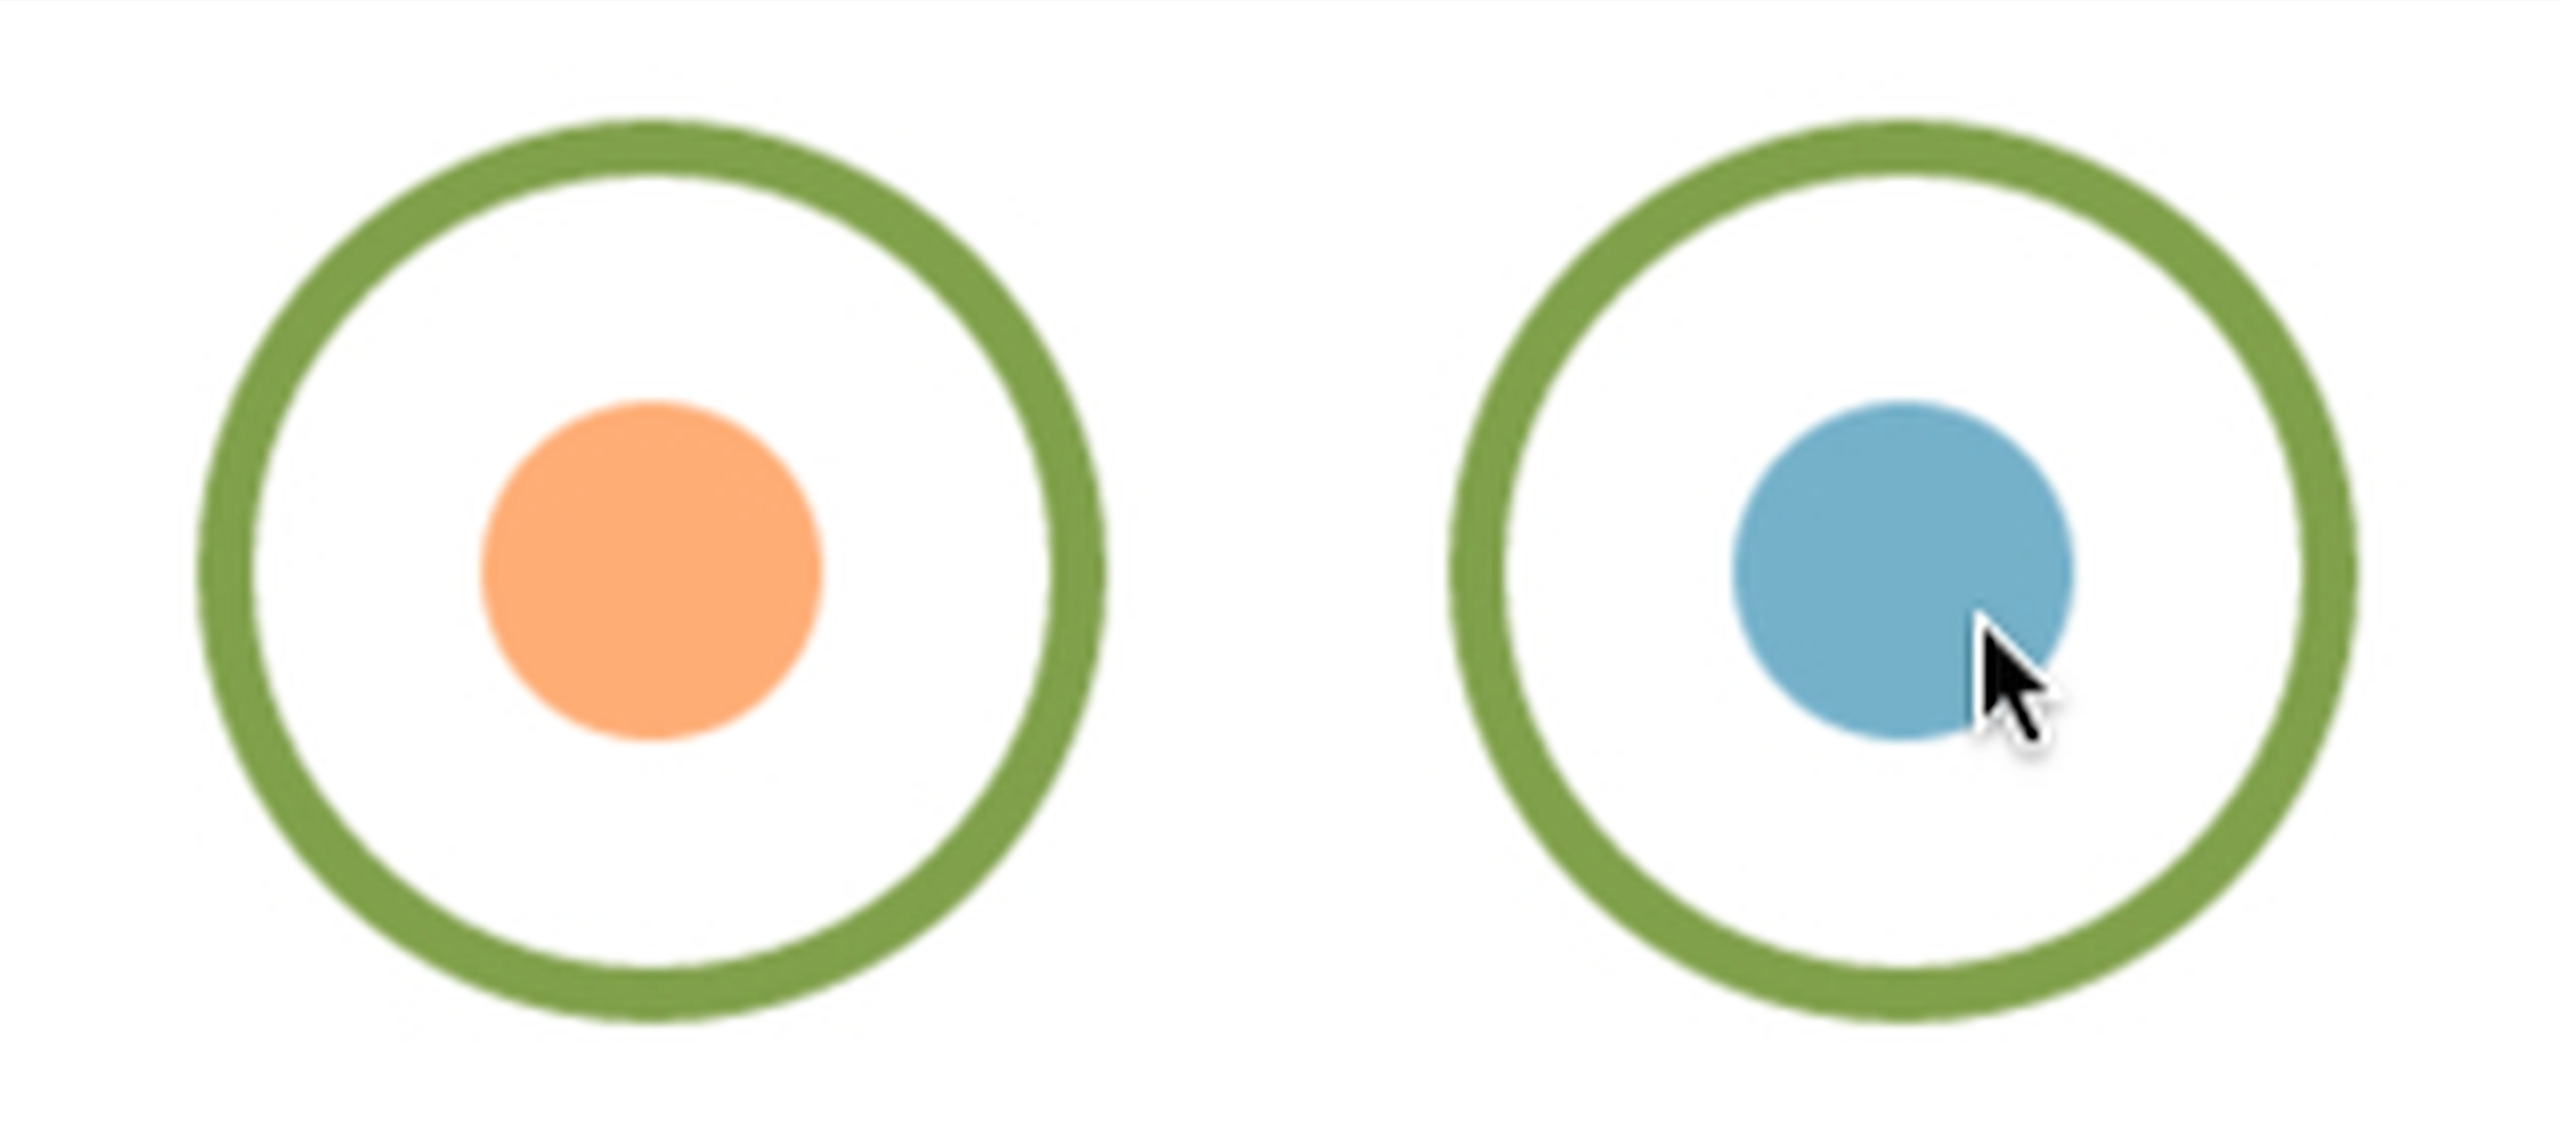
\includegraphics[width=0.6\textwidth]{joysticks}
\caption{Joysticks.}
\label{fig:joysticks}
\end{figure}


Para dotar a éste círculo de movimiento hemos utilizado los eventos de JavaScript \emph{mousedown}, \emph{mousemove}, \emph{mouseup} y \emph{mouseout}. El primer evento se ejecuta cuando el usuario hace \emph{click} con el ratón. Dentro de este evento nos encargamos de detectar si ese \emph{click} ha sido en el círculo que hemos dibujado. El segundo evento ocurre cuando, sin soltar el ratón, el usuario lo mueve. Si en el primer evento hemos detectado que ha \emph{clickado} sobre el círculo, se re-dibuja por la zona donde está moviendo el ratón. Con el evento \emph{mouseup}, al deshacer el click, re-dibujamos el círculo a su posición inicial. El evento \emph{mouseout} detecta si el ratón se ha salido del aro y también devuelve el \emph{joystick} a su posición inicial.\\

\begin{lstlisting}[caption=Movimiento y control del joystick.]
canvas.addEventListener('mousedown', function(evt) {
        var mousePos = oMousePos(canvas, evt);

        if (ctx.isPointInPath(mousePos.x, mousePos.y)) {
                arrastrar = true;
       }
}, false);

// mousemove 
canvas.addEventListener('mousemove', function(evt) {
        var m = oMousePos(canvas, evt);
        //ctx.beginPath();
        //ctx.arc(X, Y, maxR, 0, 2 * Math.PI);
        if (arrastrar) {
                delta.x = m.x - p.X;
                delta.y = m.y - p.Y;
                var deltaR = Math.sqrt(delta.x * delta.x + delta.y * delta.y);
                var elR = Math.min(deltaR, maxR);
                //console.log("DeltaR: " + deltaR + " elR: " + elR);
                var angulo = Math.atan2(delta.y, delta.x);
                //console.log(angulo); //
                
                x = X + elR * Math.cos(angulo);
                y = Y + elR * Math.sin(angulo);
                
                ctx.clearRect(0, 0, cw, ch); // Clear and redraw the joystick
                dibujarAro(X, Y, RHoop);
                dibujarCirculo(x, y, RCircle);
        }
}, false);

// mouseup 
canvas.addEventListener('mouseup', function() {
        
        sendAltYaw(0, 0);
        
        arrastrar = false;
        ctx.clearRect(0, 0, cw, ch);
        dibujarAro(X, Y, RHoop);
        dibujarCirculo(X, Y, RCircle);
}, false);

// mouseout 
canvas.addEventListener('mouseout', function() {
        sendAltYaw(0, 0);
        
        arrastrar = false;
        ctx.clearRect(0, 0, cw, ch);
        dibujarAro(X, Y, RHoop);
        dibujarCirculo(X, Y, RCircle);
}, false);
\end{lstlisting}

Dentro del evento \emph{mousemove} también recogemos la posición en la que se encuentra el \emph{joystick} y llamamos a la función correspondiente que se ocupa de enviar los datos a través del canal RTCDataChannel. En el \emph{joystick} izquierdo se llama a la función \emph{sendCMDVel()} y en el de la derecha a \emph{sendAltYaw()}.\\

Para dotar a los joysticks de funcionalidades táctiles hemos desarrollado las mismas funciones que las anteriores con los eventos táctiles equivalentes: \emph{touchstart}, \emph{touchmove}, \emph{touchend}, \emph{touchup}.\\

Estos joysticks se han situado en las esquinas inferiores de la pantalla como se puede observar en la figura \ref{fig:interfazweb} para facilitar el manejo con dispositivos táctiles.\\

\subsubsection{Gamepad}

También se ha desarrollado la posibilidad de teleoperar el drone mediante un mando USB conectado al ordenador. La API \emph{Gamepad} de JavaScript no está estabilizada, hay navegadores que no la soportan y no todos los mandos funcionan de la misma manera. El mando con el que se ha desarrollado es el \emph{Xbox} de la empresa \emph{Microsoft}, no se han realizado pruebas con mandos de otros fabricantes por lo que no se puede asegurar su correcto funcionamiento. \\

Para la detección del mando al ser conectado al puerto USB hemos usado los eventos que nos da la API \emph{Gamepad}. Al conectar el mando se ejecuta el evento \emph{gamepadconnected} que llama a la función manejadora \emph{connecthandler}.\\

\begin{lstlisting}[caption=Detección del mando.]
function connecthandler() {
    var gp = navigator.getGamepads()[0];
    console.log("Gamepad connected at index %d: %s. %d buttons, %d axes.", gp.index, gp.id, gp.buttons.length, gp.axes.length);
    updateGPInterval = setInterval(updateGamePad, 100);
    $(".joystick").fadeOut(4000);
}

window.addEventListener("gamepadconnected", connecthandler);
window.addEventListener("gamepaddisconnected", disconnecthandler);
\end{lstlisting}

La función \emph{connecthandler()} guarda en una variable el mando conectado y crea un intervalo que llama periódicamente a la función que detectará los movimientos de los botones. Por otro lado se encarga de ocultar los \emph{joysticks} virtuales, los cuales volveremos a mostrar si se desconecta el mando.\\

Dentro de la función \emph{updateGamePad()} detectamos el movimiento de los dos \emph{joysticks} del mando. y la pulsación de los botones. Hemos configurado la pulsación de una tecla para el despegue y otra para el aterrizaje, y con los \emph{joysticks} controlamos el vuelo de igual manera que con los \emph{joysticks} virtuales.\\

\begin{lstlisting}[caption=Manajador de mando.]

function updateGamePad() {
    var gp = navigator.getGamepads()[0];
    if (!gp && isChrome) {
        disconnecthandler();
        chromeInterval = setInterval(scangamepad, 1000);        
    } else {
        if (gp.buttons[0].pressed) {
            enviarOrden("takeoff");
        } else if (gp.buttons[1].pressed) {
            enviarOrden("land");
        }
        
        if (!isChrome) {
            var Y = applyDeadzone(gp.axes[0], 0.12);
            var X = applyDeadzone(gp.axes[1], 0.12);
            var Yaw = applyDeadzone(gp.axes[3], 0.12);
            var Alt = applyDeadzone(gp.axes[4], 0.12);
        } else{
            var Y = applyDeadzone(gp.axes[0], 0.12);
            var X = applyDeadzone(gp.axes[1], 0.12);
            var Yaw = applyDeadzone(gp.axes[2], 0.12);
            var Alt = applyDeadzone(gp.axes[3], 0.12);
         }
         sendCMDVel(-X*velocidad,Y*velocidad);// Change variables and send the command to the drone
         sendAltYaw(-Alt*velocidad, Yaw*velocidad);
    }
}
\end{lstlisting}

En esta función también recogemos los valores y llamamos a las funciones encargadas de enviar los datos a través del canal \emph{RTCDataChannel}.\\


\subsection{Relojes de navegación}\label{subsec:relojesnavegacion}

Para representar los datos recibidos de los sensores del drone como la altitud, velocidad, brujula, etc nos hemos ayudado de un plugin\footnote{http://sebmatton.github.io/flightindicators/}\cite{jqueryflightindicator} jQuery desarrollado por Matton Sébastien\footnote{https://github.com/sebmatton}.\\

Hemos usado cuatro relojes distintos: 

\begin{itemize}
\item Uno que nos indique la altitud del drone.
\item El segundo nos representa el horizonte.
\item El tercero es una brújula.
\item El cuarto indica la inclinación del drone.
\end{itemize}

Para crear estos relojes, creamos una etiqueta \texttt{<span>} de HTML5 para cada reloj, y posteriormente con jQuery llamamos a las siguientes funciones:\\

\begin{lstlisting}[caption=Creación de los relojes.]
var attitude = $.flightIndicator('#attitude', 'attitude', {roll:50, pitch:-20, size:s, showBox : false}); // Horizon
var heading = $.flightIndicator('#heading', 'heading', {heading:150, showBox:false, size:s}); // Compass
var altimeter = $.flightIndicator('#altimeter', 'altimeter', { showBox:false, size:s});
var turn_coordinator = $.flightIndicator('#turn_coordinator', 'turn_coordinator', {turn:0,  showBox:false, size:s}); 
\end{lstlisting}

Para actualizar los datos de estos relojes con los que llegan al par remoto directamente desde el drone se ha desarrollado una función a la que llamamos periódicamente con las variables \emph{pose} y \emph{navdata} como argumentos:\\

\begin{lstlisting}[caption=Actualización de los relojes.]
this.updatePanelControl =  function(navdata, pose){
    // calculate yaw, pitch, and roll
    var yaw = getYaw(pose.q0, pose.q1, pose.q2, pose.q3);
    var pitch = getPitch(pose.q0, pose.q1, pose.q2, pose.q3);
    var roll = getRoll(pose.q0, pose.q1, pose.q2, pose.q3);
    
    attitude.setRoll(roll);
    attitude.setPitch(-pitch);

    // Altimeter update
    altimeter.setAltitude(pose.z*100);
    //altimeter.setPressure(1000+3*Math.sin(increment/50));

    // TC update
    turn_coordinator.setTurn(roll);

    // Heading update
    heading.setHeading(yaw);
    
    // Cambiamos el ancho en el estilo del relleno de la bateria segun el nivel de bateria que nos manda el drone
    battery.style.width = String(navdata.batteryPercent) + "%";
    window.navdata = navdata;
    console.log(navdata.state);
}
\end{lstlisting}

La situación en la pantalla de estos relojes es de gran importancia. Para no ocultar la visión de la cámara y tenerlos visibles se ha decido colocarlos por pares en las esquinas superiores de la pantalla. Además, se les ha dotado de la propiedad \emph{draggable} de jQuery la cuál nos permite arrastrarlos por la pantalla y situarlos dónde más cómodo le sea al usuario.\\

\begin{lstlisting}[caption=Elementos arrastrables.]
$(function() {
    $( "#attitude").draggable();
    $( "#altimeter").draggable();
    $( "#turn_coordinator").draggable();
    $( "#heading").draggable();
});
\end{lstlisting}

En la figura \ref{fig:relojesnavegacion} podemos observar los cuatro relojes incorporados a la interfaz web de usuario. En la figura \ref{fig:interfazweb} se pueden también observar integrados con el resto de elementos que componen la interfaz.\\

\begin{figure}[h!]
\centering
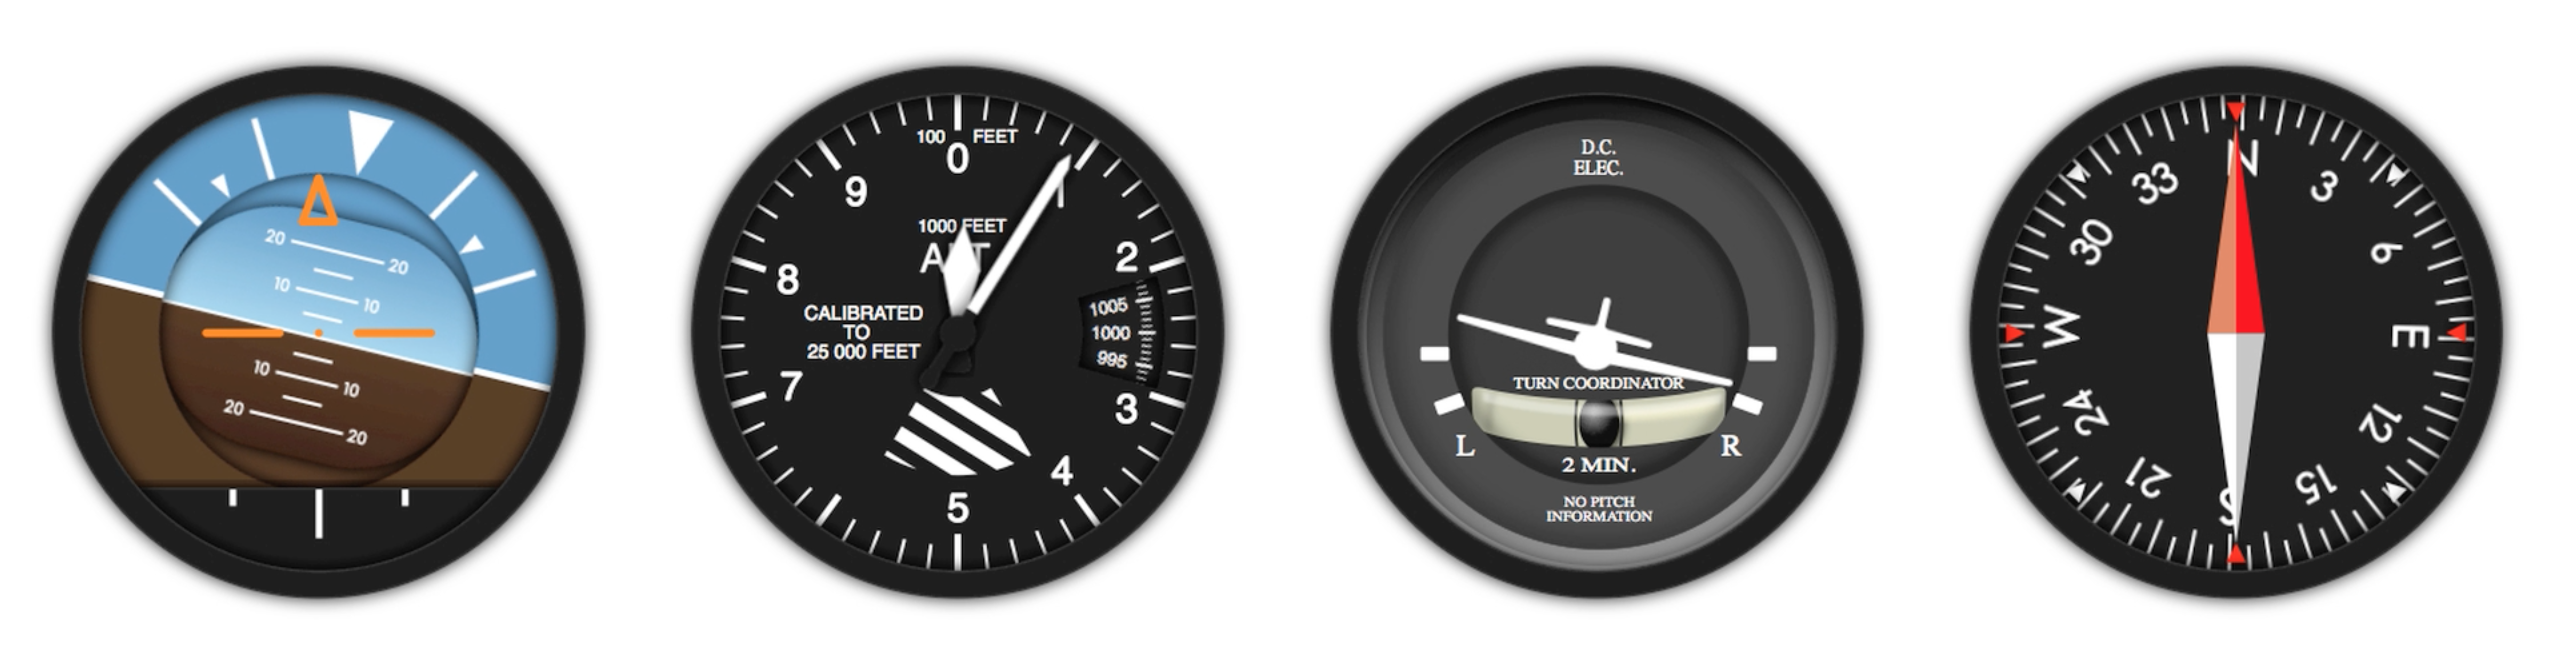
\includegraphics[width=0.9\textwidth]{relojesnavegacion}
\caption{Relojes de navegación.}
\label{fig:relojesnavegacion}
\end{figure}

\subsection{Visualización espacial 3D del drone}

Para días de niebla o condiciones extremas es imprescindible tener localizada la posición del drone para poder traerlo de vuelta. Utilizando los datos del GPS del drone hemos creado un marco 3D con la situación del drone en tiempo real. Para desarrollar este visualizador 3D nos hemos ayudado de la librería \emph{Three.js}\footnote{http://threejs.org} la cuál nos facilita el acceso y uso de WebGL. El mapa 3D es dibujado sobre una etiqueta \texttt{<canvas>}, y está compuesto principalmente por una escena, una cámara de observación en esa escena (desde ella se ve la escena), el suelo y el drone.\\

Lo primero que hemos hecho ha sido crear la escena y situar la cámara en la misma.\\

\begin{lstlisting}[caption=Escena y cámara en el mapa 3D.]
// Escena
var scene = new THREE.Scene();

//Camara
var camera = new THREE.PerspectiveCamera( 45, mapa.width/mapa.height, 0.1, 1000 );
camera.up.set( 0, 0, 1 );
camera.position.set( 18,20, 18 );
camera.lookAt( new THREE.Vector3( 0, 0, 0 )  );
\end{lstlisting}

La cámara se ha decidido que esté fija apuntando a la posición inicial del drone, ya que de esta manera es más sencillo conocer la posición del drone y devolverlo al origen si fuese necesario.\\

Posteriormente añadimos la superficie que representa el suelo con una rejilla de celdas de 1m$^{2}$.\\

\begin{lstlisting}[caption=Superficie que representa el suelo del mapa.]
// Suelo. 
var planeGeometry = new THREE.PlaneGeometry( 40, 40);
var planeMaterial = new THREE.MeshLambertMaterial( {color: 0xcccccc} );
var plane = new THREE.Mesh( planeGeometry, planeMaterial );
plane.position.x = 0;
plane.position.y = 0;
plane.position.z = 0;
plane.castShadow = false;
plane.receiveShadow = true;
scene.add( plane );
\end{lstlisting}

Three.js admite archivos en formato COLLADA \emph{(COLLAborative Design Activity)}. Hemos reutilizado los archivos Collada que utiliza el simulador Gazebo para representar de igual manera el drone. Cargamos el objeto collada del cuadricóptero, establecemos su posición inicial en el mapa y su tamaño de la siguiente manera:\\

\begin{lstlisting}[caption=Carga del objeto collada.]
var loader = new THREE.ColladaLoader();

loader.load('./collada/quadrotor/quadrotor_4.dae', function ( collada ) {
  
  dae = collada.scene;
  
  dae.position.x = 0;
  dae.position.y = 0;
  dae.position.z = 1;
  dae.scale.x = dae.scale.y = dae.scale.z = 5;
  dae.updateMatrix();
   
  daemesh = dae.children[0].children[0];
  daemesh.castShadow = true;
  daemesh.receiveShadow = true;
      
  scene.add( dae );
  render();
});
\end{lstlisting}

Desde aquí se hace también la primera llamada a la función \emph{render()} que se encargara de actualizar la posición del drone en el mapa. Este re-pintado se produce con la función \emph{requestAnimationFrame()}, la cuál admite como argumento la función a actualizar.

\begin{lstlisting}[caption=Actualización del lienzo.]
var render = function () {
  if (pose == undefined) {
    dae.position.x = 0;
    dae.position.y = 0
    dae.position.z = 0;
  }else {
    dae.quaternion.set(pose.q1, pose.q2, pose.q3, pose.q0);
    dae.position.set(pose.x, pose.y, pose.z);
      
    panelControl.updatePanelControl(navdata, pose);// update sensors watchers
  }

  renderer.render(scene, camera);
  requestAnimationFrame( render );
};
\end{lstlisting}

Para liberar al navegador de un \emph{setInterval()}, se aprovecha el 'intervalo' que crea \emph{requestAnimationFrame()} lo utilizándolo para llamar a la función \emph{updatePanelControl()} que actualiza los relojes de navegación. En la figura \ref{fig:mapa3d} se puede ver el resultado final del mapa.\\

\begin{figure}[h!]
\centering
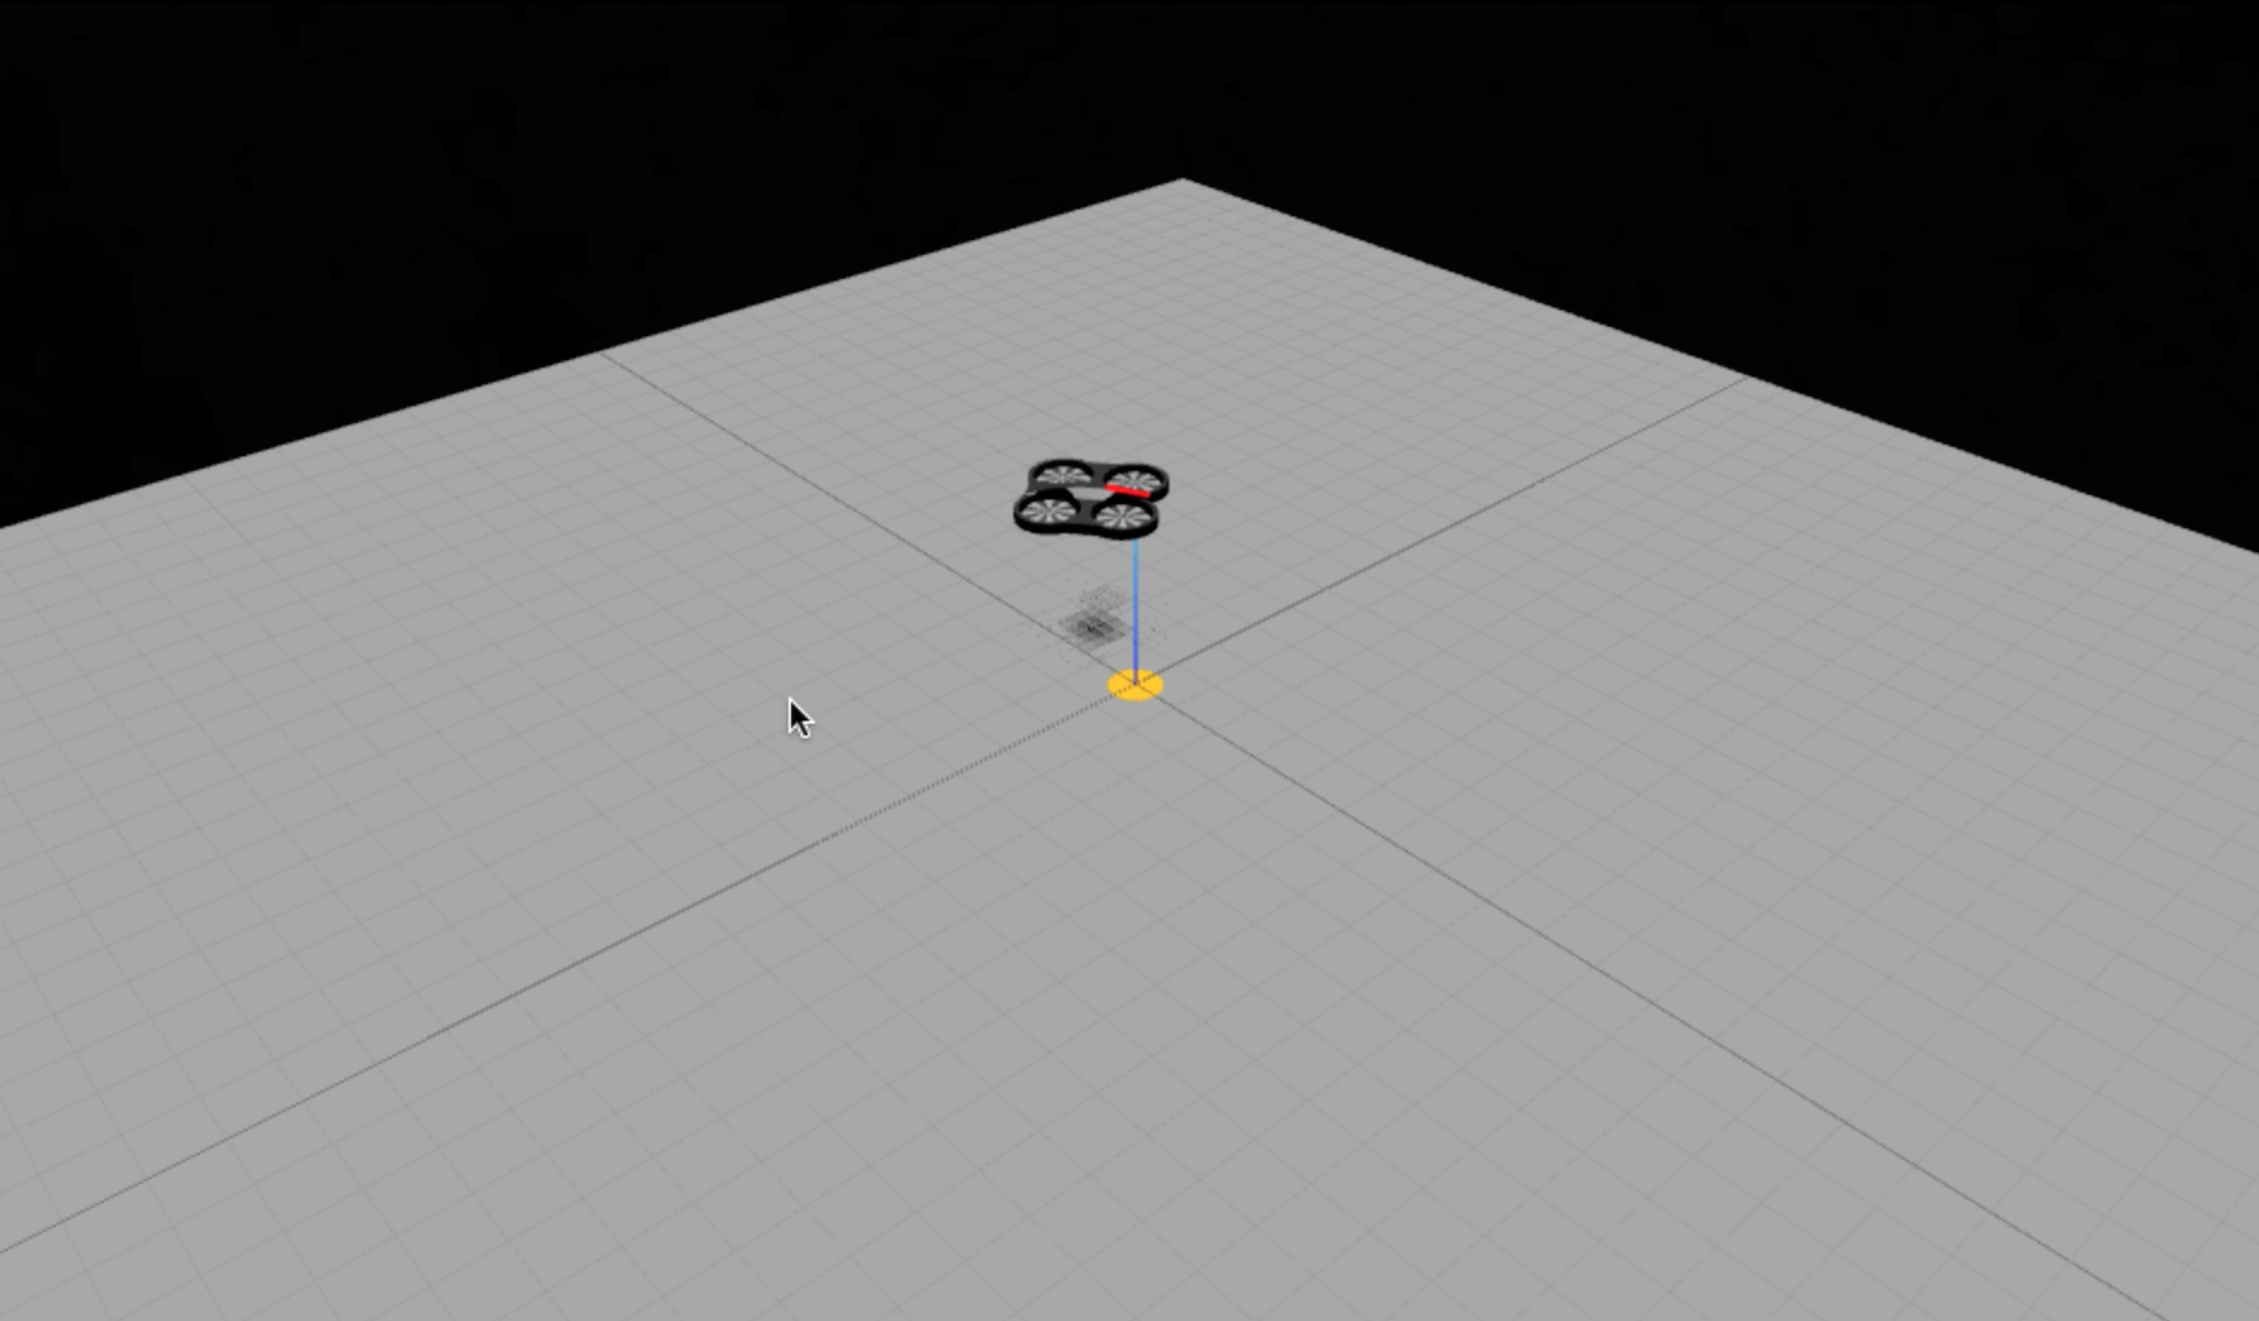
\includegraphics[width=0.6\textwidth]{mapa3d}
\caption{Mapa 3D con three.js}
\label{fig:mapa3d}
\end{figure}


Además se le han añadido dos funcionalidades más a la interfaz web. Por un lado se ha añadido un indicador de nivel de batería, creado en HTML5 y CSS3. Esta batería está desarrollada por Jon Kantner\footnote{http://codepen.io/jkantner/}\cite{bateria} y la hemos adaptado para nuestro proyecto. Por otro lado, se ha añadido un control de velocidad del drone, para facilitar su manejo si las condiciones son extremas o si se está realizando un vuelo en interiores. Este control está también desarrollado con HTML5 y CSS3 y fijan la velocidad máxima ordenable con los \emph{joysticks} visuales y el mando. Estos dos elementos están situados en la parte central superior de la pantalla como se puede ver en la figura \ref{fig:bateriayvelocidad}.\\

\begin{figure}[h!]
\centering
  \begin{subfigure}[]{60mm}
    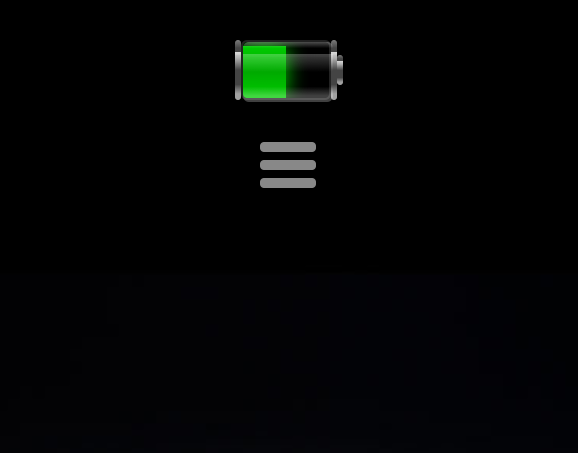
\includegraphics[width=60mm]{extras1}
    \caption{Control de velocidad sin desplegar.} 
  \end{subfigure}
  \hspace{5pt}
  \begin{subfigure}[]{60mm}
    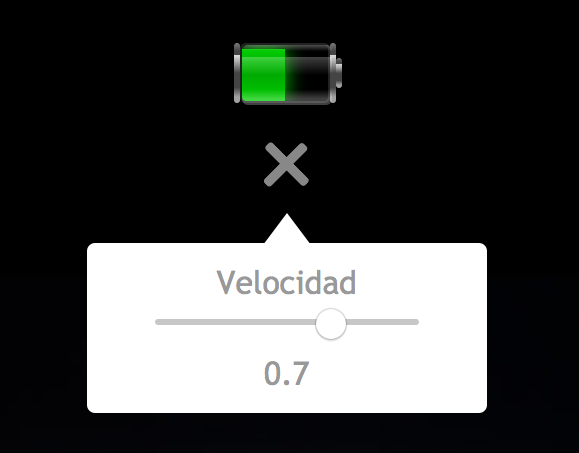
\includegraphics[width=60mm]{extras2}
    \caption{Control de velocidad desplegado.}
  \end{subfigure}
  \caption{Control de bateria y velocidad del cuadricoptero.}\label{fig:bateriayvelocidad}
\end{figure}


El resultado final de la interfaz web de usuario con todos los elementos integrados se puede ver en la figura \ref{fig:interfazweb}.


\begin{figure}[h!]
\centering
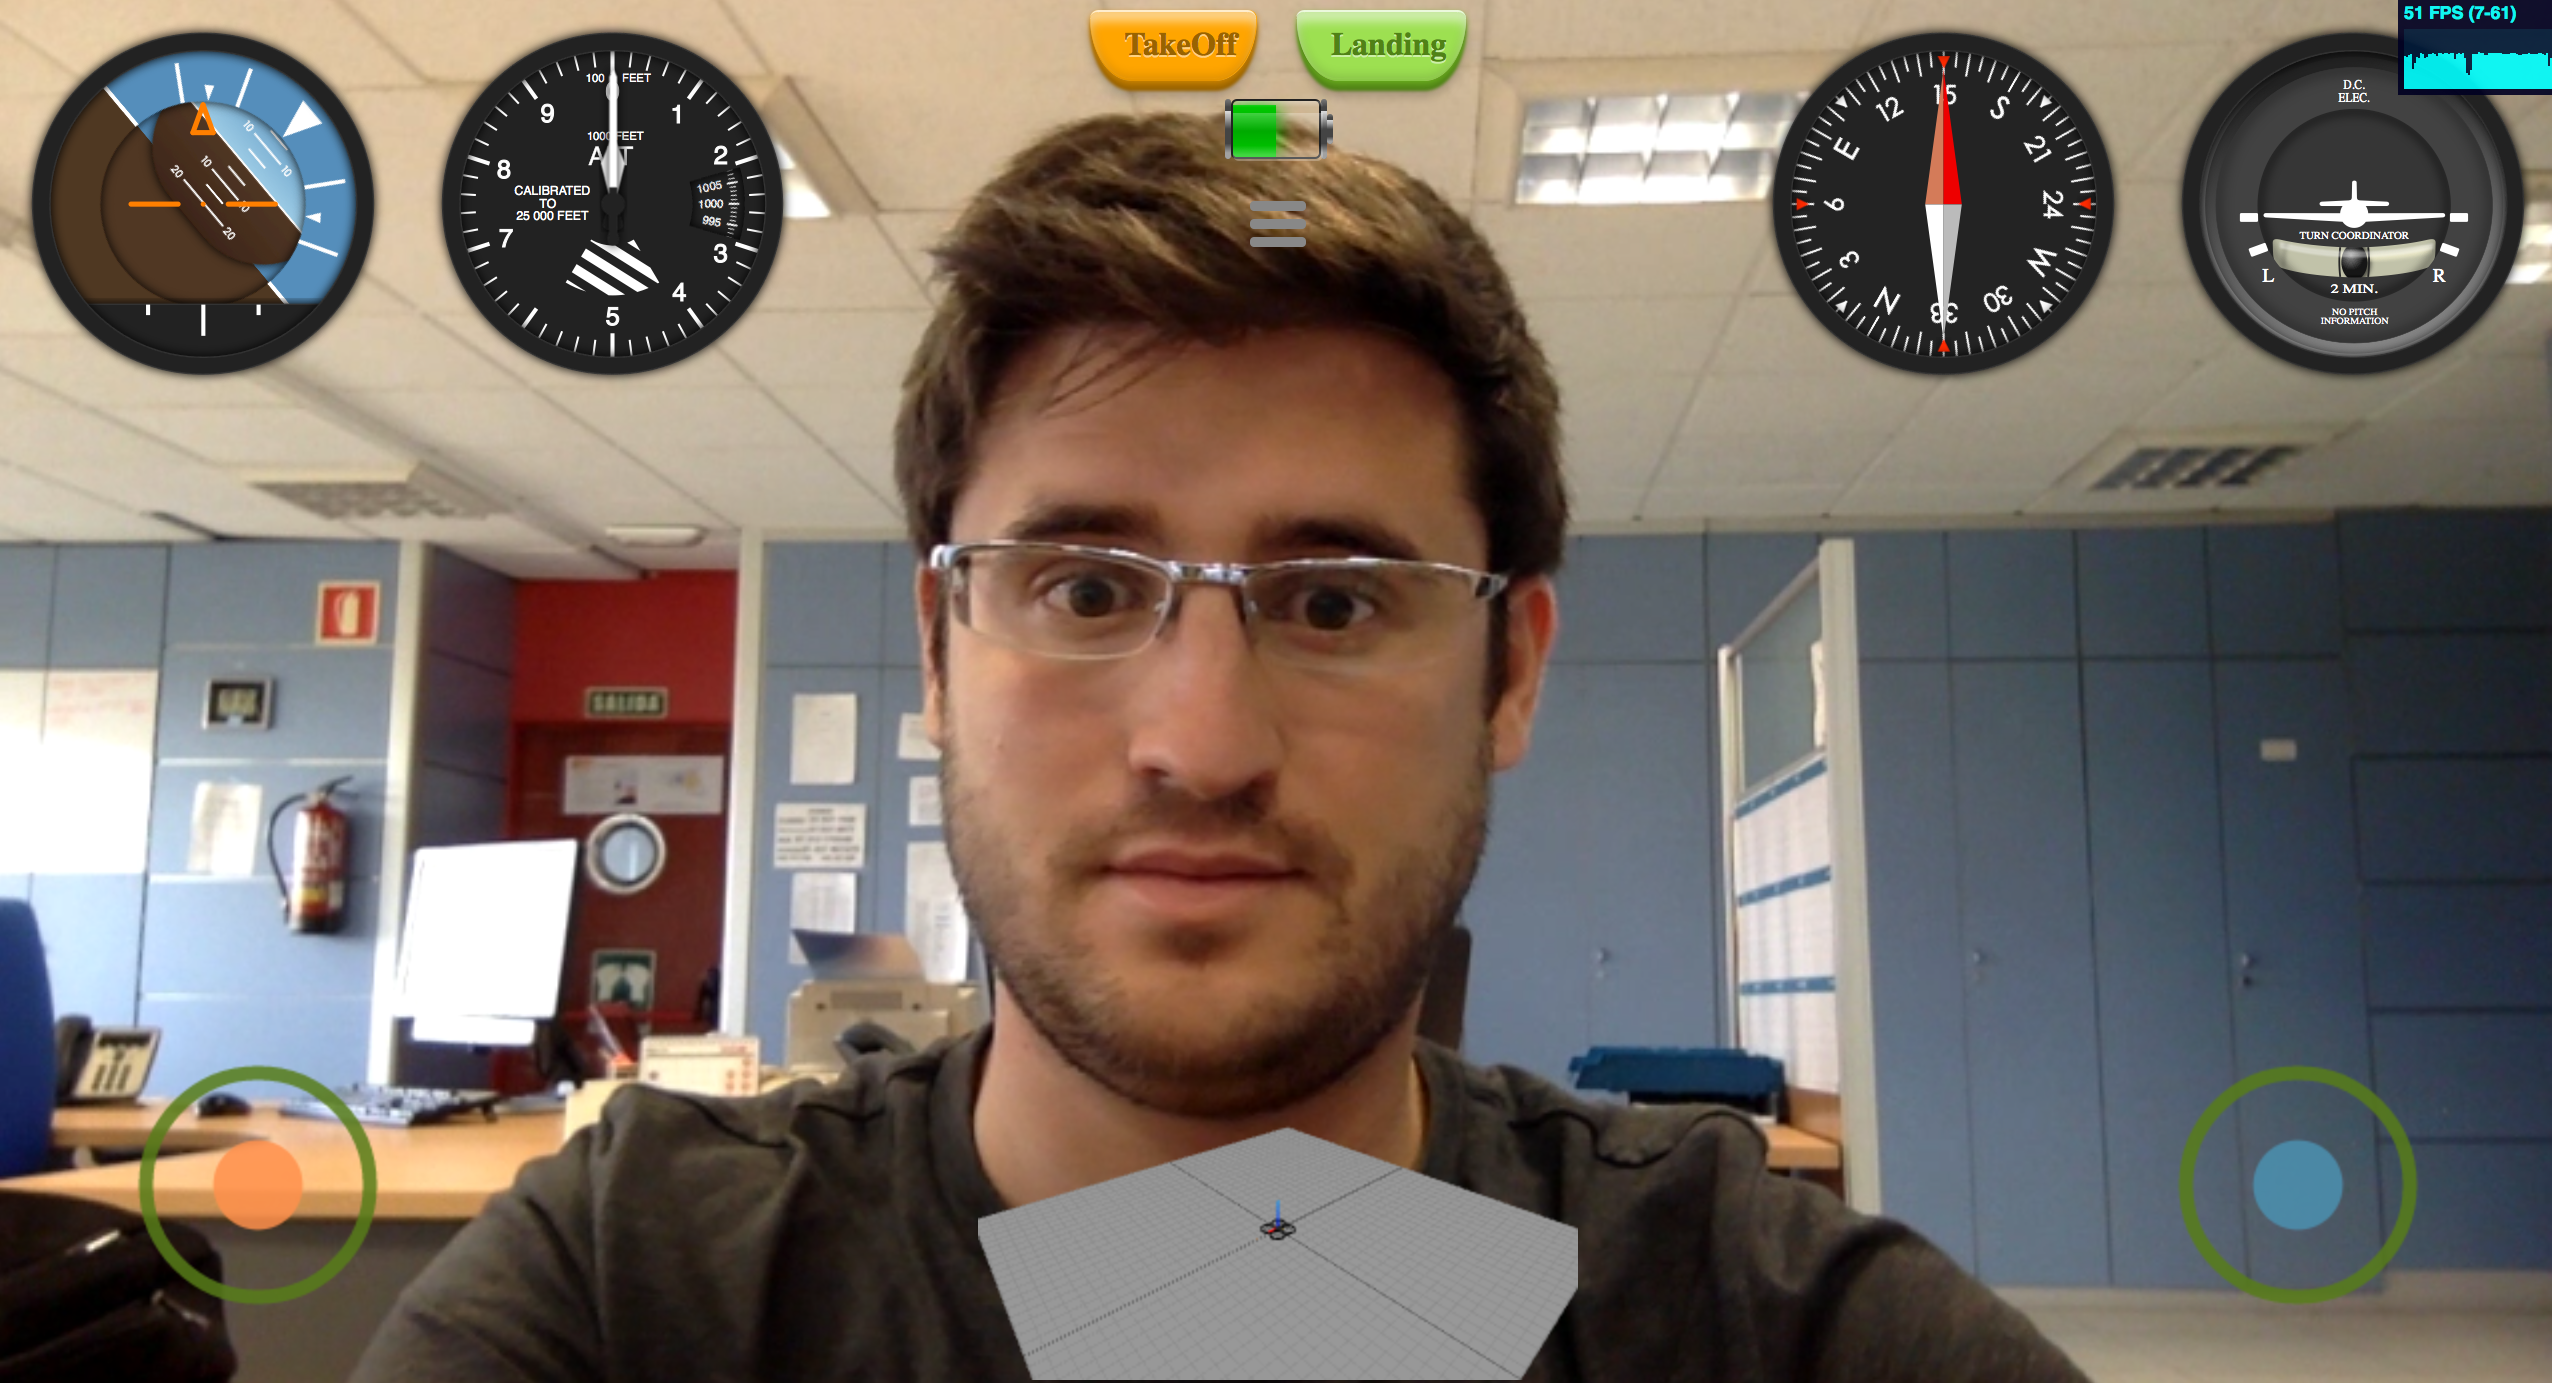
\includegraphics[width=0.9\textwidth]{interfazweb}
\caption{Interfaz web de usuario.}
\label{fig:interfazweb}
\end{figure}
